\section{The Problem}
%Knowledge vs expression intro
We have a portfolio of fixed income securities consisting of \textbf{bonds} and \textbf{swaps}. We want to understand the sensitivity of the portfolio to changes in \textbf{yields}. The \textbf{non-linear} relationship between fixed income security prices and yields, as well as a \textbf{dependence of price on the entire yield} curve makes this task more complicated than a comparable analysis of an equities portfolio. 

The value of a fixed income portfolio is a function of the cash flows due and the yield curves that discount them.  A payment from a different issuer, or due at a different time, will generally be discounted with a different yield curve.

We set two related tasks: 

First, we want a method to \textbf{simulate} the effect of changes in yield curves on a portfolio. If the 30 year treasury yield jumps by 30bps, and the BBB spread widens by 10bps at 2 years and narrows by 10bps at 10 years, we want to know what happens to the value of our portfolio.

Second, we want to be able to \textbf{attribute} changes in portfolio value to different sources. Our portfolio loses 50 million overnight -- we want to know which curve movements caused the damage. 

\section{The relationship between prices and yields }

For each borrower there is a \textbf{yield curve} of interest rates for loans of various maturities. Any bond or swap can be priced completely given the appropriate curve.

\textbf{Example: a bond} A government bond pays a 10\% coupon in one year and the face value (\$100) in two years time. The yield curve is $y(1)= 0.04$, $y(2) = 0.06$. 


The price of the bond is calculated by discounting the two cash flows (the coupon and the face value) by the appropriate yield. 

\begin{eqnarray*}
\textrm{Bond price} = \underbrace{10 \exp(-y(1)*1)}_{\textrm{Discount coupon at $y(1)$}} + \underbrace{100\exp(-y(2)*2)}_{\textrm{Discount face value at $y(2)$}}\\
=10 \exp(-0.04*1) + 100\exp(-0.06*2) = 98.3
\end{eqnarray*}

\begin{figure}[htbp]
\begin{center}
  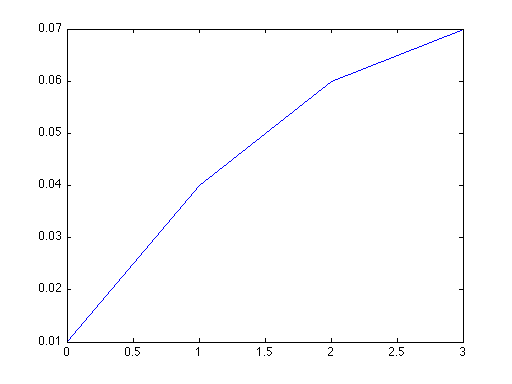
\includegraphics[width=3in]{pics/simpleYieldCurve.png} \\
  \caption{Yield curve with $y(1) = 0.04$, $y(2)=0.06$, $y(3)=0.07$}
\label{frArb}
\end{center}
\end{figure}

\textbf{Example: A swap} A swap receives the previous year's government rate $y(t-1,t)$ at $t=2,3$ and pays a fixed swap. The yield curve is $y(1) = 0.04$, $y(2) = 0.06$, and $y(3) = 0.07$. The notional value of the swap is 1 million.

The swap is priced to make the fixed and floating sides present value to zero. . The current value of the swap is the value of all remaining fixed and floating payments. This is:

\[V_{\textrm{swap}} = \sum_{\tau=2}^{3}  e^{-y(0,\tau)\tau}1M(e^{f(\tau-1,\tau)}-1 -SW) \]
 
The forward rates are

\[ f(1,2) = \frac{y(2)*2-y(1)*1}{2-1} = 0.08 \]  

\[ f(2,3) = \frac{y(3)*3-y(2)*2}{3-2} = 0.09 \]

The fair value for the swap rate is 0.088480, which is completely determined by the zero rates $y(0,t)$
%(We could also look at futures on bonds, forward rate agreements, options and so forth)


\section{Sensitivity: duration, convexity, and beyond}
How do changes in the yield curve change the value of our portfolio?

The answer depends on what kind of a change occurs in the yield curve. If all the rates on the yield curve move the same amount up or down the same amount the sensitivity will be easily described by a single number. However it's more likely that some rates will move more than others. We'll start with the simple case where everything moves the same.

\subsection{Parallel shifts in the yield curve}

Define the value of a bond as the discounted sum of cashflows

\[V = \sum_i CF_i e^{-y(t_i)t_i} \]

Now let the yield at $t_i$ be decomposed into a base yield $\bar{y}$ and an adjustment $\alpha_i$

\[V = \sum_i CF_i e^{-(\bar{y}+\alpha_i)t_i} \]

The sensitivity of the price to a simultaneous change in all the yields by the same amount is

\[ \frac{\partial V}{\partial \bar{y}} = \sum_i -t_i CF_i e^{-(\bar{y}+\alpha_i)t_i} \]

Expressing this as a percentage of value and changing the sign is 

\begin{eqnarray*}
 -\frac{1}{V}  \frac{\partial V}{\partial \bar{y}} = \frac{1}{V} \sum_i t_i CF_i e^{-y(t_i)t_i} 
 \end{eqnarray*}

This number is sometimes called the \textbf{modified duration} of the bond. Modified duration has a remarkable secondary interpretation: it's the \textbf{time weighted sum of the cashflows}.  If you imagine all the discounted cashflows on a plank representing time the this number is the location of the pivot (in time) that would make the plank balance exactly. 

\begin{figure}[htbp]
\begin{center}
  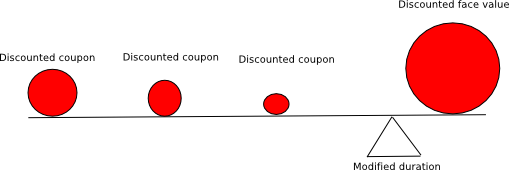
\includegraphics[width=3in]{pics/modDurn.png} \\
  \caption{Duration is the balance point of the discounted cash-flows}
\label{modDurn}
\end{center}
\end{figure}

For a zero coupon bond this is exactly equal to the maturity:

 \[-\frac{1}{V}  \frac{\partial V}{\partial \bar{y}}  = \frac{t CF e^{-y(t)t}}{CF e^{-y(t)t}} = t \]
 
 For a non-zero coupon bond this will be somewhat less than the maturity. 
 
\begin{figure}[htbp]
\begin{center}
  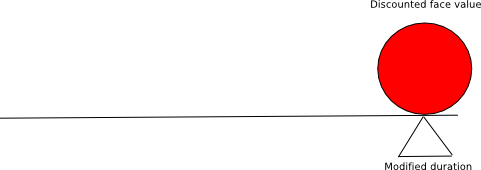
\includegraphics[width=3in]{pics/modDurnZc.png} \\
  \caption{Modified duration of a zero coupon bond is the maturity }
\label{modDurnZc}
\end{center}
\end{figure}
 
Duration is useful because it gives a sense of how large a move in the price of the bond will arise from a shift in yields. If the yield curve shifts up by 1\% the price of a 2 year treasury bond will not move much, the price of a 30 year treasury bond will move drastically. 

Duration is also \textit{additive} over a portfolio. We can add up all durations of each security in the portfolio to get the total first order sensitivity. 

The problem with duration is that it only answers a very specific question: ``what happens to the price of a bond when the yield curve shifts uniformly?" The number is a summary of the effects of each yield on each cashflow of the bond. We could get an better picture by looking at the effect of changes at any point on the curve. Duration is a useful summary, but it can only ever be an approximate measure of interest rate sensitivity.  


\textbf{Example: Duration of a bond}
Returning to the simple bond of the previous example, and with the same yield curve, the duration is

\[ \frac{1*10 \exp(-0.04*1) + 2*100\exp(-0.06*2)}{98.3} = 1.9023  \] 

The \textbf{dollar duration} is the same but without dividing by the bond price

\begin{eqnarray*}
\frac{\partial V}{\partial \bar{y}} = \sum_i -t_i CF_i e^{-(\bar{y}+\alpha_i)t_i}\\
  = -1*10 \exp(-0.04*1) + -2*100\exp(-0.06*2) = -1.87 
 \end{eqnarray*}

This means the price of the bond will change by approximately  \$1.87  for a 0.01 move in the interest rate. This is approximate because the price is not a linear function of the yield, so the duration will itself change with the yield. The change is larger if the yield curve is lower.

We can trace out the change in sensitivity for a range of yield curves:

\begin{center}
\begin{tabular}{|c|c|c|c|}
\hline
$y(1)$ & $y(2)$ & duration & dollar duration\\
\hline
0.02& 0.04 & 1.904 &-1.94\\
0.03 & 0.04 &1.903 &-1.91\\
\textbf{0.04} & \textbf{0.06} & \textbf{1.902} & \textbf{-1.87} \\
0.05 & 0.07 & 1.901&-1.83\\
0.06 & 0.08 & 1.900 &-1.8\\
\hline
\end{tabular}
\end{center}

\textbf{Example: Duration of a swap}
Consider again the swap from the earlier example. Swap duration involves two complications. First, since the swap is priced correctly it has no `value' as would a bond, so it is impossible to divide by $V$ in the usual duration calculation. We must therefore use \textbf{dollar duration}. Second, the value of the floating cashflows are valued using forward rates, and so are also sensitive to movements in the yield curve. Normal bonds don't have this problem because all cashflows are fixed.

It's not a huge problem. All we do is note that each cashflow $CF_i$ of the swap is now also a function of the \textit{level} of yields $\bar{y}$. 

\[V_{\textrm{swap}} = \sum_i CF_i(\bar{y}) e^{-y(t_i)t_i} \]

The dollar duration is then given by the product rule

\begin{eqnarray*}
\frac{\partial V}{\partial \bar{y}}  =  \sum_i -t_i CF_i(\bar{y}) e^{-y(t_i)t_i} + \frac{\partial CF_i(\bar{y})}{\partial \bar{y}} e^{-y(t_i)t_i} \\
\end{eqnarray*}

Recall that the arbitrage free price of the cashflow is 

\[CF_i = N(e^{f(t_i-1,t_i)}-1-SW)  \]

Where $N$ is the notional value and $SW$ is the swap rate. The one period forward price has the same sensitivity to to $\bar{y}$ as any zero rate so the duration of the swap is

\begin{eqnarray*}
 \frac{\partial V_{\textrm{swap}}}{\partial \bar{y}}  = \sum_i -t_i N(e^{f(t_i-1,t_i)}-1-SW) e^{-y(t_i)t_i} + e^{f(t_i-1,t)} e^{-y(t_i)t_i} \\
 = -2*1M (e^{f(1,2)}-1-SW )e^{-y(2)*2} +  e^{f(1,2)}e^{-y(2)*2}  +\\
  -3*1M (e^{f(2,3)}-1-SW )e^{-y(3)*3} +  e^{f(2,3)}e^{-y(3)*3} \\ 
 = -2*1M (e^{0.08}-1-0.0885 )e^{-0.06*2} +  e^{0.08}e^{-0.06*2}  +\\
  -3*1M (e^{0.09}-1-0.0885 )e^{-0.07*3} +  e^{0.09}e^{-0.07*3} \\ 
 = 4635.5\\
\end{eqnarray*}

So, approximately, a 0.1\% upward shift in all yields will cost the swap-holder \$46.36. 

\subsection{Second order sensitivities and other measures}
Most fixed income securities do not have a linear payoff in yield: the duration changes as the yields change. Also yield curves rarely shift in neat parallel movements. To get a broader picture we need higher order sensitivities.

The second order sensitivity is called the \textbf{convexity}. If the cashflows are not a function of the yield this is

\[ \frac{\partial^2 V}{(\partial \bar{y})^2} =  \sum_i t_i^2 CF_i e^{-y(t_i)t_i}  \] 
 
 If cashflows are a function of yields (as with a vanilla swap) we have
 
 \[\frac{\partial V}{\partial \bar{y}}  =  \sum_i -t_i CF_i e^{-y(t_i)t_i} + \frac{\partial CF_i(\bar{y})}{\partial \bar{y}} e^{-y(t_i)t_i} \]
 
 so
 
  \[\frac{\partial^2 V}{(\partial \bar{y})^2}  =  \sum_i t_i^2 CF_i e^{-y(t_i)t_i} + \frac{\partial^2 CF_i(\bar{y})}{(\partial \bar{y})^2} e^{-y(t_i)t_i} - t_i\frac{\partial CF_i}{\partial \bar{y}}e^{-y(t_i)t_i} \]


This is the \textbf{dollar convexity}. If we want to express the convexity as a proportion of the price we can divide by $V$. Convexity is a useful measure as it shows how quickly the duration is changing. A portfolio with high convexity can be very risky as portfolio sensitivities can quickly accelerate.


\section{Simulation and attribution}

\subsection{Breaking it down}
Fixed income portfolios will typically have a number of bonds (and swaps and futures and options) from various issuers and at various maturities. As yield curves shift the value of the portfolio changes.  \textbf{Attribution} is the process of decomposing the sources of these changes in price.

The purpose of the process is to gain an insight into where our returns are coming from. If we make \$20 on our portfolio we want to know how much of that is due to changes in the 10 year treasury yield, and how much due to the change in the 2 year BBB spread on treasuries. 

A sensible way to do this is to break down the zero rate on each issuer into a number of components. For example the two year zero rate for a particular BBB issuer is the 2 year government rate plus the 2 year credit spread. 

\begin{figure}[htbp]
\begin{center}
  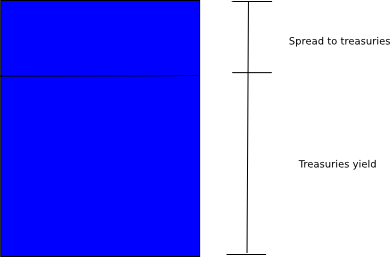
\includegraphics[width=3in]{pics/yCurveDec1.png} \\
  \caption{Yield = treasuries yield + spread}
\label{yCurveDec1}
\end{center}
\end{figure}

We can drill down further if we like: the two year government rate is the real rate plus inflation. (If there is a market for inflation swaps we can know this exactly). The credit spread for a particular BBB issuer is the BBB reference rate plus or minus the spread for that issuer against the reference rate. 

\begin{figure}[htbp]
\begin{center}
  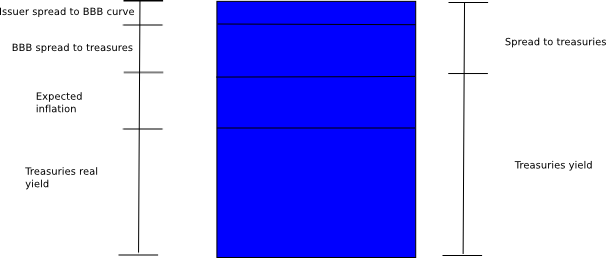
\includegraphics[width=3in]{pics/yCurveDec2.png} \\
  \caption{Yield = treasuries yield + spread = treasuries real yield + expected inflation + BBB spread to treasuries + issuer spread to BBB}
\label{yCurveDec1}
\end{center}
\end{figure}

For an issuer $a$, $y_a(t)$ is the zero rate for maturity $t$. The return to a portfolio can be approximately broken down to the changes in each of these components, as well as the passage of time.

\[y_a(t) = y_{\textrm{real treasury yield}}(t) + y_{\textrm{inflation}}(t) + y_{\textrm{reference yield for issuer $a$}}(t) + y_{\textrm{spread of issuer $a$ to reference yield}}(t)\]

Or any other decomposition of interest. 


\subsection{First principles or perturbation?}
For a given change in all the components of each zero rate $y_a(t)$ to a new curve $y_a'(t)$ we can determine the change in the value of a portfolio by comparing the value of each cashflow at the old yield and new yield. The sum of these changes will be the total change in the value of a the portfolio. 

\[ V = \sum_a \sum_i CF_i^a \exp(-y_a(t)t)\]

So for a change in a particular yield $y_a(t)$ to $y_a^{'}(t)$ 

\[ \Delta V = \sum_a \sum_i CF_i^a \exp(-y_a(t)t) - \sum_a \sum_i CF_i^a \exp(-y_a'(t)t)  \]

We then sum over all $a$ to give the total portfolio change. We can also divide up the yield into its components and trace the change in portfolio value due to each yield change. This is called the \textbf{first principles} approach.

Alternatively we can take a Taylor series expansion for each yield

\[ \Delta V = \frac{\partial V}{\partial y_a(t)}  (y_a(t)-y_a'(t)) + \frac{1}{2}\frac{\partial^2 V}{\partial y_a(t)^2} (y_a(t)-y_a'(t))^2 + O((y_a(t)-y_a'(t))^3) \]

(where $O((y_a(t)-y_a'(t))^3)$ denotes a series of terms that are at most of order $(y_a(t)-y_a'(t))^3$ -- namely quite small so we ignore them)

This is called the \textbf{perturbation} approach.

The advantage of the perturbation approach is that it allows us to express the change in value in terms of duration and convexity without worrying about every cash flow. This gives a very compact (though slightly approximate due to removing higher order terms) summary of the sensitivity of the portfolio to changes in particular yields, or to parallel shifts in any of the curves.

\textbf{Attribution example}

Let's say we have a portfolio of 1 treasury bond and 1 corporate bond issued by B-Corp. Both bonds have a maturity of two years, a face value of \$100, and pay a 10\% coupon after 1 year. 

We have two relevant yield curves: the treasury curve, and the B-Corp curve. It is useful to think of the B-Corp curve as a spread to treasuries (the additional yield on B-corp debt over same maturity treasury debt). Suppose the curves are initially thus:

\begin{tabular}{|c|c|c|}
\hline
 Period & 1 & 2\\
 \hline
Treasury & 0.03 & 0.03\\
B-Corp spread to treasuries & 0.03 & 0.03\\
\hline
\end{tabular}

The total yield on 1 year B-Corp shares is then the rate on treasuries plus the spread (0.03+0.03 = 0.06). We can price the portfolio by the discounted cash flows:

\[ V = \underbrace{10 \exp(-0.03*1)+ 100 \exp(-0.03*2)}_{\textrm{Treasury bond}} + \underbrace{10\exp(-0.06*1)+ 100 \exp(-0.06*2)}_{\textrm{B-Corp bond}} = 201.99\]

 All at once the treasury yield curve shifts up by 100bps, as does the B-Corp credit spread. 

\begin{tabular}{|c|c|c|}
\hline
 & 1 & 2\\
 \hline
Treasury & 0.04 & 0.04\\
B-Corp spread to treasuries & 0.04 & 0.04\\
\hline
\end{tabular}

The revised portfolio price is 

\[ V = \underbrace{10 \exp(-0.04*1)+ 100 \exp(-0.04*2)}_{\textrm{Treasury bond}} + \underbrace{10\exp(-0.08*1)+ 100 \exp(-0.08*2)}_{\textrm{B-Corp bond}} = 196.37\]

The portfolio value has decreased by \$5.63. How does this break down?

Using the first principles approach we can price each cash flow under the old ($y$) and new ($y'$) yield curves. 

\begin{tiny}
\begin{tabular}{|c|cc|c|cc|c|}
\hline
 & & y&  & & y' & \\
 Maturity & 1 & 2 & $\Sigma$ & 1 & 2 & $\Sigma$ \\
 \hline
Treasury bond & $10e^{-0.03*1} = 9.70$  & $100e^{-0.03*2}=94.18$ & 103.88 & $10e^{-0.04*1} = 9.61$ & $100e^{-0.04*2}=92.31$ & 101.92\\
B-Corp Bond & $10e^{-0.06*1} = 9.42$ & $100e^{-0.06*2}= 88.69$ & 98.11 & $10e^{-0.08*1}=9.23$ & $100e^{-0.08*2}=85.21$ & 94.45\\
\hline
 & & & 201.99 & & & 196.37\\
 \hline
\end{tabular}
\end{tiny}

Under the first yield curve the portfolio is worth  103.88 + 98.11 = 201.99.  Under the second the portfolio is worth 101.92+ 94.45 =196.37 . The difference is 5.62 (we accumulated -0.01 due to rounding). 

How much of this is due to the shift in the treasuries curve and how much to the shift in the B-Corp curve? The surprising answer is that it depends which way you look at it. 

Let's say the treasury curve shifts first from $y(1) = y(2) = 0.03$ to $y(1) = y(2) = 0.04$. This pushes the B-Corp curve from $y(1) = y(2) = 0.06$ to $y(1) = y(2) = 0.07$. Then the shift in B-Corp spread pushes the B-Corp curve to $y(1) = y(2) = 0.08$.

If the B-Corp spread moves first then the B-Corp curves moves from $y(1) = y(2) = 0.06$ to $y(1) = y(2) = 0.07$. The shift in treasuries moves it up to $y(1) = y(2) = 0.07$ to $y(1) = y(2) = 0.08$.

In both cases the treasury is first worth 103.88 and then 101.92 (a change of -1.96).  However in the first case the treasuries shift decreases the price of the B-Corp bond from 98.11 to 96.25 (a change of -1.85); and in the second case from 96.25 to 94.45 (a change of -1.81). The difference is due to the convexity of the bond. The sensitivity to a 100bps shift in yields is lower after a shift has already occurred.

At still higher prevailing levels of B-Corp yields the difference would be smaller still as we see in the table below.

\begin{tabular}{|c|c|}
\hline
level of B-Corp yields & change in B-Corp bond price after 1\% increase in yields\\
\hline
0.06 & -1.85\\
0.07 & -1.81\\
0.08 & -1.78\\
0.09 & -1.74\\
0.1 & -1.71\\
\hline
\end{tabular}


The 4 cent difference might seem like small beans but for larger yield moves and at longer maturities these differences become significant. In practice attribution must simply follow a convention: For instance we might measure the impact of the treasury curve first and the B-Corp spread afterwards.

Now let's try the perturbation approach. Recall that we can approximate the change in value arising from changes in yields by the first two terms of the Taylor series.

\[ \Delta V \simeq \frac{\partial V}{\partial y_a(t)}  (y_a(t)-y_a'(t)) + \frac{1}{2}\frac{\partial^2 V}{\partial y_a(t)^2} (y_a(t)-y_a'(t))^2  \]

The relevant terms for both bonds in each period are below:

\begin{tabular}{|c|cc|cc|}
\hline
 Issuer & &  Government bond & & B-Corp\\
 Period & 1 & 2 & 1 & 2\\
 \hline
 $\frac{\partial V}{\partial y(t)}$ & -9.70 & -188.35 & -9.42 & -177.38\\
 $\frac{\partial^2 V}{\partial y(t)^2}$& 9.70 & 376.71& 9.42 & 354.77\\
 $\Delta y(t)$ & 0.01 & 0.01 & 0.02 & 0.02\\
 $(\Delta y(t))^2$  & 0.001 & 0.001 & 0.004 & 0.004\\
 $\Delta V \simeq \frac{\partial V}{\partial y(t)} + \frac{1}{2} \frac{\partial^2 V}{\partial y(t)^2}(\Delta y(t))^2$ & -0.0966 & -1.8647 &  -0.1865 & -3.4767\\
 \hline
 \end{tabular}

From this we can see the total anticipated change in the government bond price is -0.0966 -1.8647 = -1.9613, and the anticipated change in the B-Corp bond is   -0.1865 -3.4767 = -3.6632. Both are around what we expect.

The table also shows us the effect of the price from movements in different parts of the curve. The value of the \$10 coupon on the government bond moves -0.0966 due to a 0.01 increase in y(1); the value of the \$100 at maturity moves -1.8647 due to the 0.01 increase in y(2). 

This table allows us to estimate other changes too. By changing the row with $\Delta y(t)$  we can accommodate any change in the structure of the yield curve.

We still have the question of how much of the change is due to the change in the government curve and how much to the change in the B-Corp spread. Again the answer depends which change we consider first. One approach is to consider more `primitive' moves first: we consider a change in the government rate before a change in the BBB reference rate; and  that before a change in the B-Corp spread to the reference rate.

Reality is more complicated than this simple example. Bonds pay irregular coupons; not all points on the yield curve are available or reliable; some bonds embed options for early repayment, which complicates matters. There are other complexities too. But the basic process is quite simple. We have a series of zero curves which can be used to price known future cash flows. As the curves move the cashflows must be repriced. Sensitivities change. The rest is detail.

%Higher order Taylor series and Taylor series involving time.\\ An integral representation \\Appendix on Taylor series?

\section{A general schema for fixed income portfolio management}

Take a step back. We know a few things:

\begin{enumerate}
\item  Every potential borrower (including you and I) has a yield curve giving the market interest rate of loans at all maturities. 
\item Each of these rates can be decomposed into a risk free part (proxied by government rates) and a credit part (the difference between each rate and government rate). We can break rates down further by splitting government rates into real rates and expected inflation, and credit spreads into reference rates for certain classes of credit and spreads to those reference rates. Or any other decomposition of interest.  
\item Each fixed income security is a series of cashflows due at some future time. The value of those cashflows is determined by discounting them by the rate (yield) for that issuer at that maturity.
\item When yield curves shift the value of these discounted cashflows change. We can \textbf{attribute} these changes by  recalculating the value of the securities at the old and new yields. Because different yield curves have common components we can vary the components one at a time, and observe how much each change affects the value 
\item We follow the same process to determine the effect of hypothetical changes in yield curves\\
\item The total effect of a change in yields can be well estimated by the first two terms in a Taylor series of the value of a each cashflow as a function of its yield.
\end{enumerate}

A general representation of a fixed income portfolio is then 

\begin{eqnarray*}
V = \sum_a \int CF_a(t)e^{-y_a(t)t}dt \\
y_a(t) = \omega_a' c(t)
\end{eqnarray*}

Where $CF_a(t)$ is a cashflow from issuer (borrower) $a$ in period $t$ and $y_a(t)$ is the yield for issuer $a$ for loans with maturity $t$. 

We decompose $y_a(t) = \omega_a' c(t)$ where $c(t)$ is a vector of component yields and $\omega_a$ is a vector of weights of each of the component yields for issuer $a$. This allows us to calculate the effect of each component yield on the total portfolio. For most cases the components of $c(t)$ will be \textbf{orthogonal} so $\frac{\partial c_i(t)}{\partial c_j(t)} = 0$ for $i \neq j$.  

For example if the compenents were 

\[c(t) = (y_{\textrm{treasuries}}(t),y_{\textrm{B-Corp spread to treasuries}}(t))\] 

Then weight vector for treasury bonds would be $\omega_{\textrm{treasures}} = [1, 0]$, and for B-Corp bonds $\omega_{\textrm{B-Corp bonds}} = [1,1]$.

We can derive all first and second order sensitivities easily. The results are for fixed cashflows. Extending to cases where the cashflow is a function of yields (for instance if swaps are involved) is straightforward but a little messier.

\begin{eqnarray*}
\frac{\partial V}{\partial y_a(t)} = \sum_a -t CF_a(t) e^{-y_a(t)t}\\
\frac{\partial^2 V}{\partial y_a(t)^2} = \sum_a t^2 CF_a(t) e^{-y_a(t)t}\\
\frac{\partial V}{\partial c_i(t)} = \sum_a -\omega_a(i) t CF_a(t) e^{-y_a(t)t}\\
\frac{\partial^2 V}{\partial c_i(t)^2} = \sum_a \omega_a(i)^2t^2 CF_a(t) e^{-y_a(t)t}
\end{eqnarray*}

Sensitivities to the \textbf{levels} of individual yield curves $y_a(t)$ or to the \textbf{components} $c_i(t)$ (call these $\bar{y_a}$ and $\bar{c_i}$) are straightforward:

\begin{eqnarray*}
\frac{\partial V}{\partial \bar{y_a}} = \int_0^{\infty}\frac{\partial V}{\partial y_a(t)}dt\\
\frac{\partial^2 V}{\partial \bar{y_a}^2} = \int_0^{\infty}\frac{\partial^2 V}{\partial y_a(t)^2}dt\\
\frac{\partial V}{\partial \bar{c_i}} = \int_0^{\infty}\frac{\partial V}{\partial c_i(t)}dt\\
\frac{\partial^2 V}{\partial \bar{c_i}^2} = \int_0^{\infty}\frac{\partial^2 V}{\partial c_i(t)^2}dt\\
\end{eqnarray*}


\section{Questions}

\textbf{Question 1}\\

A bond pays a \$5 coupon at $t=0.5$ and a \$100 coupon at $t=50$. Yields are $y(0.5) = 0.01$ and $y(50) = 0.02$.

\begin{tabular}{l}
(a) What is the modified duration and convexity of the bond?\\
(b) What is the dollar duration of a:\\
\begin{tabular}{l}
(i)  100bps downward shift in the yield curve\\
(ii) 100bps downward movement in y(0.5)\\
(iii) 100bps downward movement in y(50)\\
\end{tabular}\\
(c) Calculate the expected change in price from using a first principles approach and a Taylor series approximation.
\end{tabular}

\medskip

\textbf{Question 2}\\

Say the yield curve is  $y(0.5) = 0.01$, $y(1) = 0.01$, $y(50) = 0.02$, $y(51) = 0.02$

The sway pays y(0.5,1)*1M at $t=1$ and $y(50,51)*1M$ at t=51 and receives a fixed swap rate.

\begin{tabular}{l}
(a) What is the appropriate swap rate?\\
(b) What is the dollar duration of the swap?\\
\end{tabular}

\medskip

\textbf{Question 3}\\

Reconsider the bond in question 1. This bond is issued by B-Corp. B-Corp yields can be decomposed into a treasuries component and a spread. Say the curves move as in the table below. How much of the change in yields can be attributed to the change in the treasuries curve and how much to the change in the B-Corp spread?


\begin{tabular}{|c|c|c|c|c|}
\hline
 & & y&  & y'  \\
 Maturity & 0.5 & 50 & 0.5 & 50 \\
 \hline
Treasury bond (bps) & 75 & 150 & -25 & 100 \\
B-Corp spread (bps) & 25 & 50 & 25 & 0\\   
 \hline
\end{tabular}
%\end{block}



%Contract specifications
%Pricing
%Decomposing yields (inflation/credit/etc)
%Duration of a bond future/option



